\section{实验评估}
\label{sec:exp_belief}

本节评估信念表征网络在不同任务中的实证表现，包括确定性和随机环境。
在\Cref{subsec:setting_exp_belief}中描述每个任务、基线方法和 D-TRPO 的设定。
在\Cref{subsec:results_belief}中提供并讨论实验结果。

\subsection{设定}
\label{subsec:setting_exp_belief}

注意，所有基线、本文方法和所有任务的结果均在 10 个随机种子下取平均。

\subsubsection{任务}
\label{subsubsec:tasks}
\noindent\textbf{Pendulum.}\indent 在该任务中，智能体必须学习将钟摆向上旋转。
该任务是延迟\gls{rl}中的经典任务，因为传统\gls{rl}算法的性能随延迟增大而迅速下降。
部分原因在于上方位置的不稳定平衡点，在延迟情况下难以维持。
在实现中，使用 \texttt{gym} 库~\cite{brockman2016gym}的版本。
该环境是确定性的。
鉴于在 Pendulum 上运行实验的计算成本相对较低，我们对集合 $\{3, 5, 10, 15, 20\}$ 中的常值延迟重复分析。
对该任务，执行 500 轮（epoch），每轮 5,000 步，总计 250 万步。

\noindent\textbf{随机 Pendulum.}\indent 该任务与前一个任务相同，但人为地向过程添加随机性。
具体而言，向智能体选择的动作添加形式为 $\epsilon = \text{scale}( \eta+ \text{shift})$ 的独立同分布噪声，其中 $\eta$ 为某个概率分布。
\Cref{tab:noises}给出了考虑的六种噪声。
还考虑一种额外噪声：环境以 0.9 的概率遵循智能体指示的动作，否则均匀随机采样一个动作。
将此过程称为\emph{均匀}（uniform）噪声。
对这些任务，仅考虑延迟为 5，执行 1,000 轮，每轮 5,000 步，总计 500 万步。

\begin{table}[t]
\centering
    \begin{tabular}{|l||l|l|l|l|}
        \hline
        Noise & Distribution  $\eta$ & Shift & Scale & Group \\ \hline
        \textit{Beta (8,2)}& $\beta (8,2)$ & $0.5$ & $2$ &  1\\
        \textit{Beta (2,2)} & $\beta (2,2)$ & $0.5$ & $2$ & 1\\
        \textit{U-Shaped} & $\beta (0.5,0.5)$ & $0.5$ & $2$ & 1\\
        \textit{Triangular} & $\text{Triangular} (-2,1,2)$ & $0$ & $1$ & 2\\
        % \textit{Uniform} & $\text{U} (-1,1)$ & $0$ & $1$ & 2\\
        \textit{Lognormal (1)} & $\text{Lognormal} (0,1)$ & $-1$ & $1$ & 3\\
        \textit{Lognormal (0.1)} & $\text{Lognormal} (0,0.1)$ & $-1$ & $1$ & 3\\
        \hline
    \end{tabular}
    \caption{随机 Pendulum 中动作添加噪声的分布。}
    \label{tab:noises}
\end{table}

\noindent\textbf{Mujoco.}\indent 这是一个连续机器人运动控制任务，使用 \texttt{mujoco}~\cite{todorov2012mujoco} 库提供的高级物理模拟器。
这些任务的复杂性在于其复杂的动力学以及大状态和动作空间。
从所有 Mujoco 环境中，考虑 Walker2d、HalfCheetah、Reacher 和 Swimmer，这些环境在早期测试后证明受延迟影响最大。
与 Pendulum 类似，这可以用某些情况下存在不稳定平衡点来解释。
这些环境是确定性的。
对这些任务，仅考虑延迟为 5，执行 1,000 轮，每轮 5,000 步，总计 500 万步。


\subsubsection{基线方法}
\label{subsubsec:baselines}
作为基线，包括基于增广状态的 \gls{trpo}（A-TRPO）和无记忆 \gls{trpo}（M-TRPO），以覆盖基于 \gls{trpo} 的方法谱系。
此外，考虑 \gls{sac}，因其在延迟应用中取得了优异的实证结果\cite{ramstedt2019real,bouteiller2020reinforcement}。
还在基线中包括基于增广状态的 \gls{sac}（A-SAC）和无记忆 \gls{sac}（M-SAC）。
\gls{sac} 的一个超参数是其更新频率。
尽管将该参数设置为每一步都重新训练可提高样本效率，但会显著增加计算时间和内存占用。
因此，仅在 Pendulum 上每一步都训练 \gls{sac}，而在 Mujoco 上限制为每 50 步训练一次以加速过程。
曾考虑加入 DCAC~\cite{bouteiller2020reinforcement}，但其实现计算开销较大，决定不纳入。
早期实验结果表明其运行时间超过其他算法的 10 倍以上。
此外，考虑 SARSA 和 $\lambda=0.9$ 的 dSARSA，但仅用于 Pendulum 环境。由于 SARSA 是一种批量\gls{rl}算法，需要对状态和动作空间进行仔细离散化，这直接影响最终性能。
因此，需要额外的离散化验证步骤。
对 Pendulum，使用经过调优的 15x15 状态空间网格和总共五个离散动作。
最后，在测试中将 L2-TRPO 作为基线，该方法采用与\cite{firoiu2018human}类似的方法学习状态的期望值。


\subsubsection{D-TRPO 的设定}
在呈现的实验中，测试 D-TRPO，即信念表征网络接入\gls{trpo}~\cite{schulman2015trust}后的结果。
一个重要说明是，经过 D-TRPO 的早期实验，我们注意到信念模块优化过程中信念表征可能发生显著变化。
这反过来导致 \gls{trpo} 策略优化不稳定，因为其输入分布不断变化。
为缓解此问题，在 200 轮后提前停止信念表征模块的训练。


\subsection{结果}
\label{subsec:results_belief}

\begin{figure}[t]
    \centering
    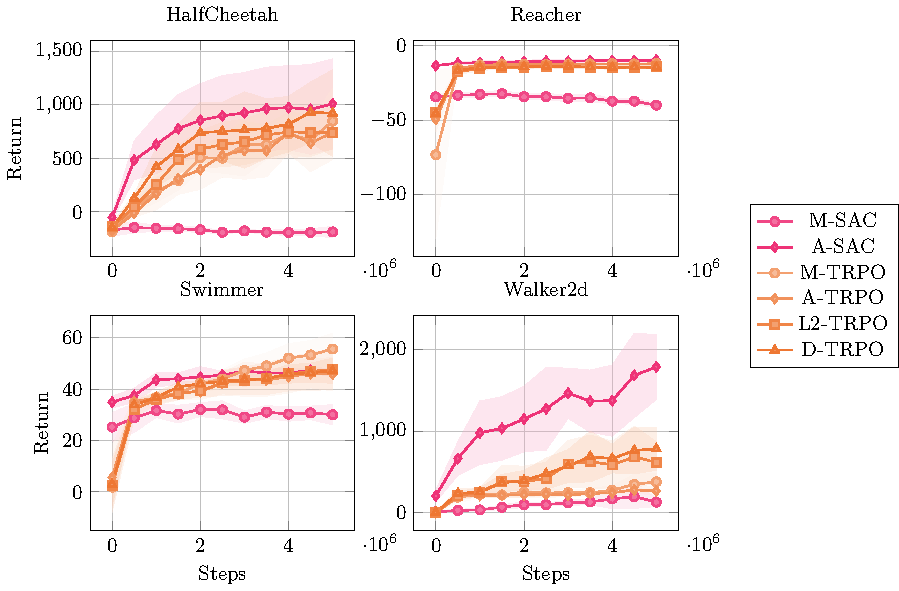
\includegraphics[labelbelief=pendulumvaryingdelay]{img/thesis_plots_belief.pdf}
    \caption{Pendulum 环境中 D-TRPO 和基线方法在不同延迟值下的平均回报。
    水平虚线表示无延迟 \gls{sac} 的性能。
    阴影区域表示一个标准差，结果基于 10 个随机种子获得。}
    \label{fig:pendulum_varying_delay_belief}
\end{figure}

\noindent\textbf{Pendulum.}\indent 不同方法和不同延迟值下的回报见\Cref{fig:pendulum_varying_delay_imitation}。
水平虚线表示无延迟版本 \gls{sac} 获得的回报。
对于不超过五的延迟，D-TRPO 和 L2-TRPO 的回报与无延迟 \gls{sac} 相当。
同时注意 A-SAC 在此情况下的优异表现。
然而，随着延迟增加，D-TRPO 和 L2-TRPO 的性能下降比 A-SAC 更显著。
在\Cref{fig:delay_5_pendulum_belief}中，聚焦延迟为 5 时 D-TRPO 和基线方法在学习阶段的表现。
图中还报告了无延迟 \gls{trpo} 的结果。自然，后者比任何基于 \gls{trpo} 的延迟方法更快，但有趣的是，它比 A-SAC 慢。
这表明 SAC 在解决此问题时特别有效，即便存在延迟。
除 A-SAC 外，D-TRPO 和 L2-TRPO 具有最快的收敛速度，与无延迟 TRPO 相比，需要额外约 100 万步才能达到类似策略。



\begin{figure}[t]
    \centering
    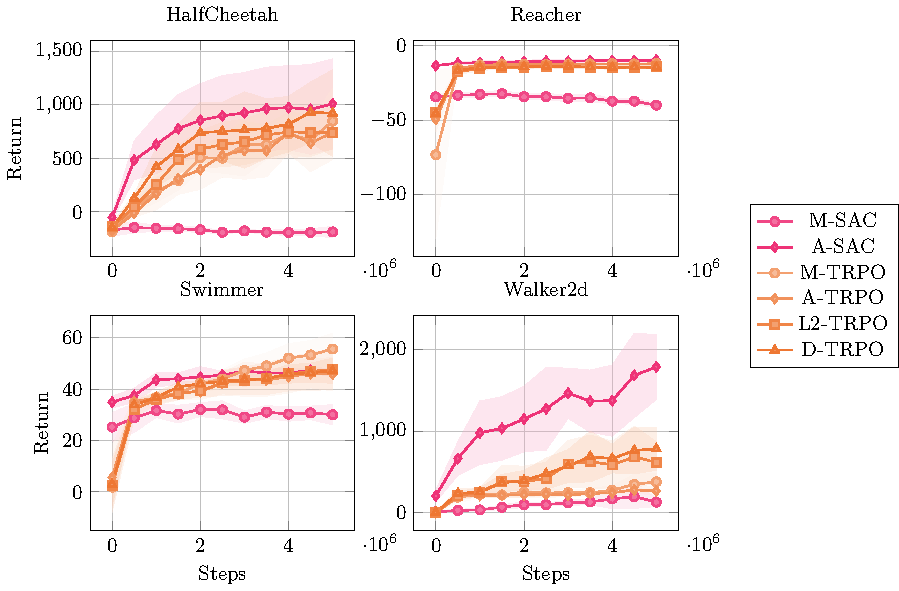
\includegraphics[labelbelief=delay5pendulumbelief]{img/thesis_plots_belief.pdf}
    \caption{D-TRPO 和 L2-TRPO 与延迟为 5 的 Pendulum 任务中其他基线方法的回报比较。包含无延迟 \gls{trpo} 的性能（记为``TRPO'')作为对照。
    阴影区域表示一个标准差，结果基于 10 个随机种子获得。}
    \label{fig:delay_5_pendulum_belief}
\end{figure}

\noindent\textbf{Mujoco.}\indent 在\Cref{fig:delay_5_mujoco_belief}中，报告 Mujoco 环境的结果。
此处同样，A-SAC 特别高效，仅在 Swimmer 环境中未获第一。
令人惊讶的是，在 500 万步后，M-TRPO 在该环境中表现最佳。
D-TRPO 和 L2-TRPO 在所有环境中表现良好，仅在 Walker2d 上出现明显性能不足。

\begin{figure}[t]
    \centering
    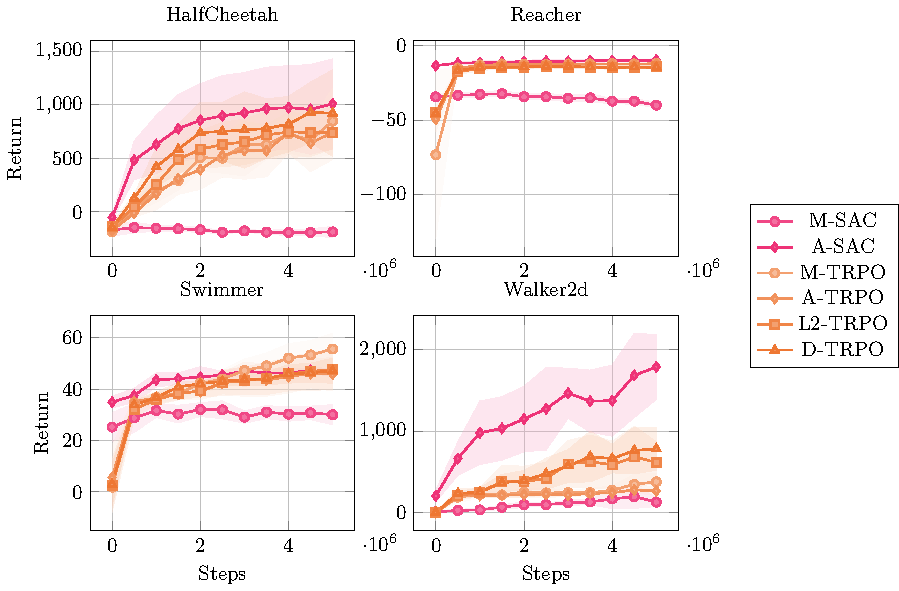
\includegraphics[labelbelief=delayfivemujocobelief]{img/thesis_plots_belief.pdf}
    \caption{D-TRPO 和 L2-TRPO 与基线方法在各种 Mujoco 环境中的回报比较。
    阴影区域表示一个标准差，结果基于 10 个随机种子获得。}
    \label{fig:delay_5_mujoco_belief}
\end{figure}

\noindent\textbf{随机 Pendulum.}\indent 在该任务上，仅比较 D-TRPO 与 L2-TRPO，以评估学习未来状态信念表征相对于其均值的优势。
结果报告在\Cref{fig:delay_5_pendulum_noise_belief}中。
为便于阅读结果，将噪声分为三组。
可以观察到 D-TRPO 从未被 L2-TRPO 超越。
对于某些噪声类型，如 Uniform 和 Triangular 噪声，两者获得相似的性能。
然而，对于其他类型的噪声，如 Quadratic 和 LogNormal (0.1) 情况，性能差异更为明显。
这表明信念表征在最坏情况下并非必要，但在最佳情况下可提供更高性能。

\begin{figure}[t]
    \centering
    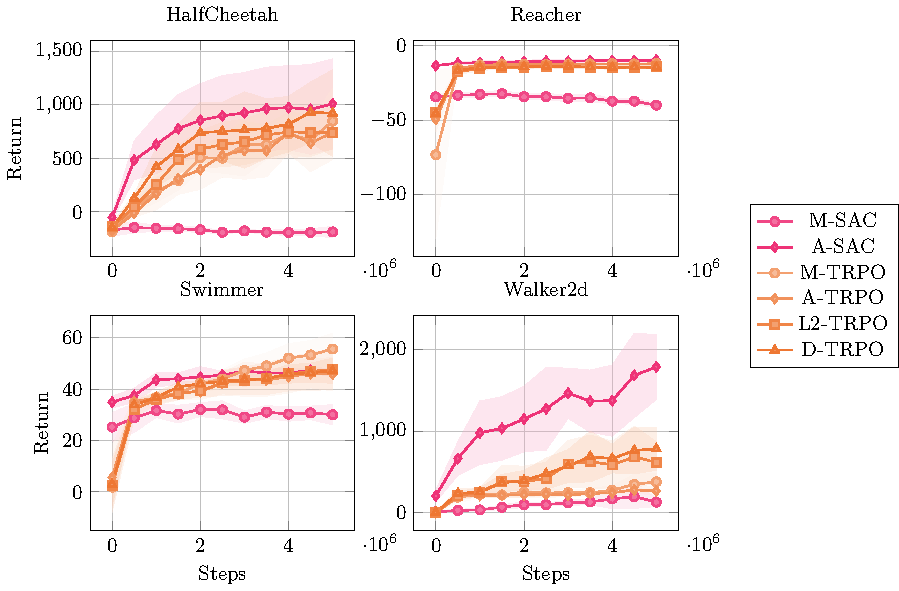
\includegraphics[labelbelief=pendulumnoisebelief]{img/thesis_plots_belief.pdf}
    \caption{D-TRPO 和 L2-TRPO 与基线方法在添加不同噪声（如\Cref{tab:noises}所述）的 Pendulum 环境中的回报比较。
    颜色表示噪声类型，标记表示算法。
    阴影区域表示一个标准差，结果基于 10 个随机种子获得。}
    \label{fig:delay_5_pendulum_noise_belief}
\end{figure}


\noindent\textbf{同时学习多个延迟.}\indent
\label{subsec:learning_multi_delay_once_belief}
在该实验中，测试\Cref{subsec:multi_delay_once_belief}中提出的思路，即 D-TRPO 和 L2-TRPO 在某个延迟 $\delay>0$ 下学习的策略应用于另一个延迟 $0<\delay'<\delay$。
在\Cref{fig:multi_delay_pendulum_dtrpo}中，提供 Pendulum 任务上 D-TRPO 和 L2-TRPO 以 $\delay=5$ 训练的结果。
在\Cref{fig:multi_delay_mujoco_dtrpo}和\Cref{fig:multi_delay_mujoco_ltrpo}中，提供 Mujoco 任务上 D-TRPO 和 L2-TRPO 以 $\delay=5$ 训练的结果。
显然且符合预期，较小延迟下获得的性能与原始性能相当。

\begin{figure}[t]
    \centering    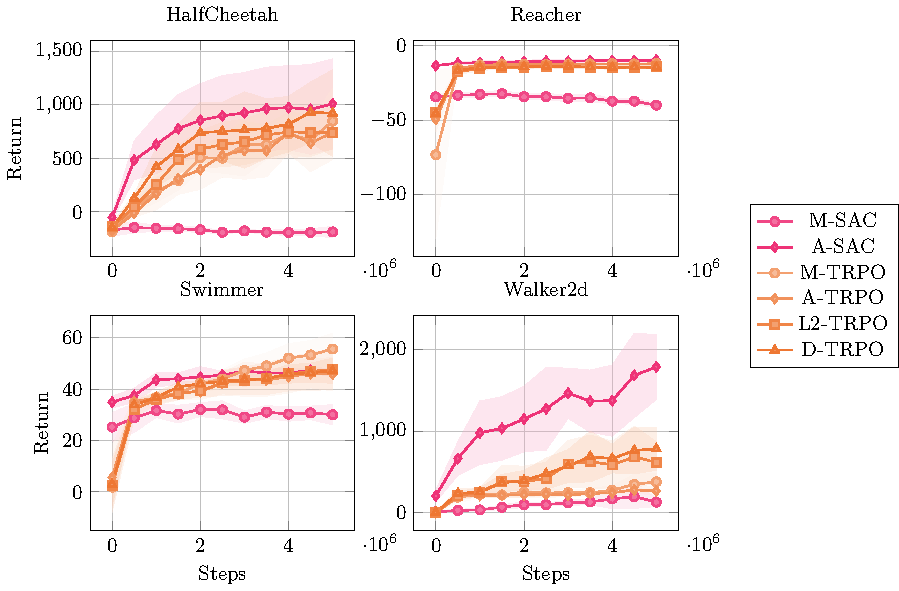
\includegraphics[labelbelief=multipledelayspendulumdtrpo]{img/thesis_plots_belief.pdf}
    \caption{延迟 10 训练的 D-TRPO 在 Pendulum 上以更小延迟测试的回报。}
    \label{fig:multi_delay_pendulum_dtrpo}
\end{figure}

\begin{figure}[t]
    \centering
    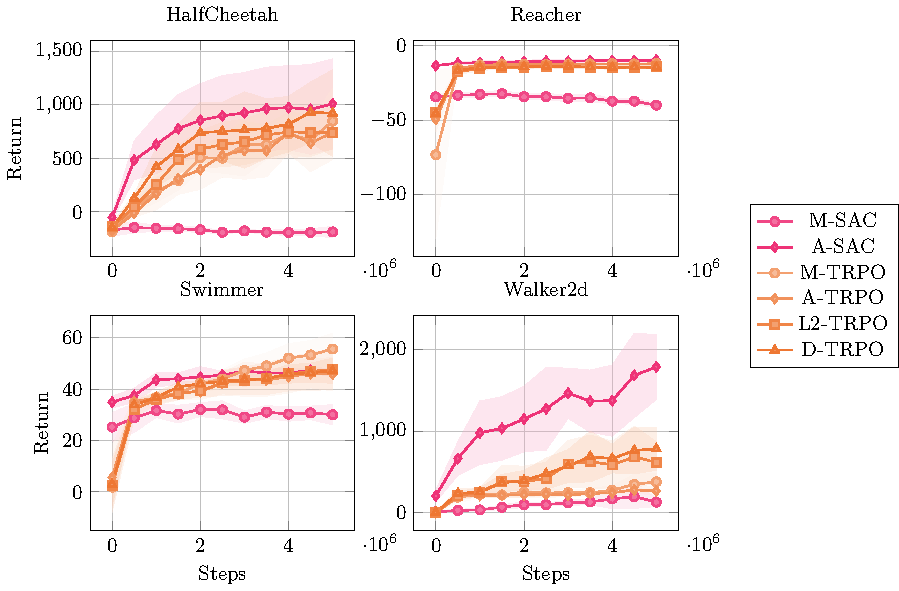
\includegraphics[labelbelief=multipledelaysmujocodtrpo]{img/thesis_plots_belief.pdf}
    \caption{延迟 5 训练的 D-TRPO 在 Mujoco 环境中以更小延迟测试的回报。}
    \label{fig:multi_delay_mujoco_dtrpo}
\end{figure}

\begin{figure}[t]
    \centering
    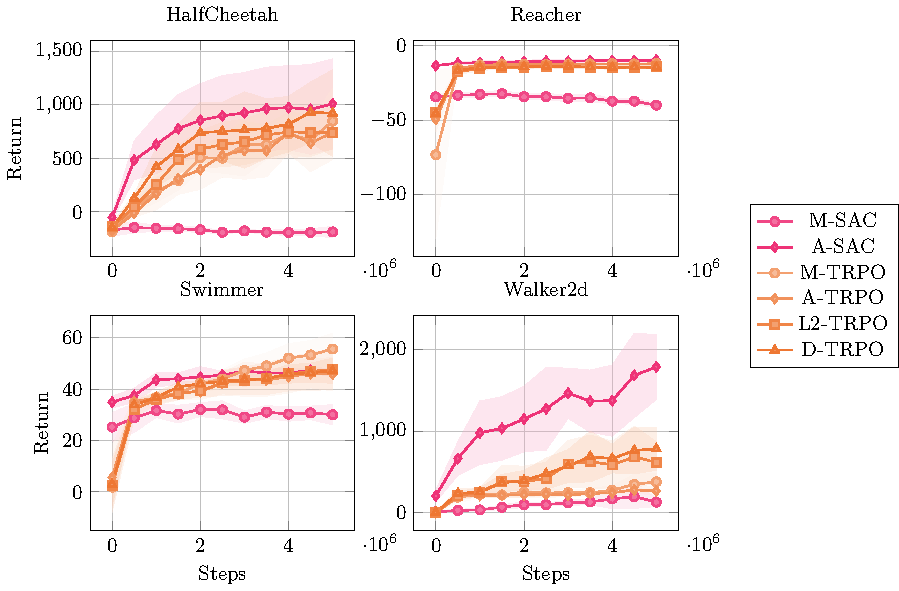
\includegraphics[labelbelief=multipledelaysmujocoltwotrpo]{img/thesis_plots_belief.pdf}
    \caption{延迟 5 训练的 L2-TRPO 在 Mujoco 环境中以更小延迟测试的回报。}
    \label{fig:multi_delay_mujoco_ltrpo}
\end{figure}
